%        File: report.tex
%     Created: Tue Jun 09 02:00 PM 2015 C
% Last Change: Tue Jun 09 02:00 PM 2015 C
%
\documentclass[12pt]{scrreprt}
\usepackage[utf8]{inputenc}
\usepackage [backend=bibtex]{biblatex}
\addbibresource{bibliography.bib}
\usepackage{graphicx}
\graphicspath{ {images/} }
\usepackage[autostyle]{csquotes}
\usepackage{caption}
\usepackage{subcaption}
\usepackage{mathtools}
\usepackage{listings}
\begin{document}
% Title Page
\author{Miłosz Mazur}
\title{Cooperation Evolved}
\subtitle{Behavior Trees evolution by means of Genetic Programming}
\maketitle

\newpage
\chapter*{Abstract}
Behavior Trees are a method for AI programming that consists of a tree of hierarchical nodes controlling the flow of agent's decision making. They have proven, while being a pretty straightforward means to implement an AI, to be incredibly powerful way of obtaining autonomous agents, both due to a fact that the development can be iterable (one can start with implementing simple behavior and gradually improve the tree by adding and modifying nodes and branches) and allowing for, so to say, ``fallback tactics'', should the currently executed action fail.  Born in the game industry, they have since gained fair amount of popularity in other domains, including robotics.
Evolutionary algorithms, largely popularized by John Holland \cite{hollandadaptation}, have been adapted for use in a vast variety of different problems, including optimization issues and decision handling, often through introducing serious changes to both the algorithm structure and data structures used. Arguably, one of the most valuable modifications was Genetic Programming, popularized through works of John Koza (\cite{kozagp}).

This thesis documents the work on combining Behavior Trees and Genetic Programming in order to study and observe cooperative and adversative behaviors between agents controlled by genetically generated Behavior Trees. Evolving two kinds of agents in two contrasting scenarios, this thesis focuses on \textit{feasibility} of cooperation and its evolution.  % two sentences about scenarios

\chapter*{Acknowledgements}
\input{chapters/acknowledgements}
\tableofcontents
\listoffigures
\listoftables
\chapter{Introduction}
\label{chapter_introduction}
\section{Thesis Goal}
The main goal of the thesis is to answer the question:
%``Can we teach artificial agents to cooperate by forcibly putting them in conflicting situations?''
``How cooperative behaviors between artificial agents influence the performance in multi-agent task-oriented environments?'' % efficiency?
\section{Thesis Research Goals}
\begin{itemize}
    \item Provide a platform that can be used to automatically generate and evaluate artificial agents.
    \item Measure and find a way to deal with the impact of the initial generation.
    \item Measure the effect cooperative behaviors had on task execution.
\end{itemize}
\section{Challenge}
The true challenge in presented work is to provide a valid way to compare two drastically different approaches to the task in order to prove whether changing said approach is tied to a change in efficiency of the task's execution. Before the grounds for the comparison can be defined, a common goal must be stated for agents in both approaches, thus formulating aforementioned task.

The technical challenge, on the other hand, is in applying genetic operators to a delicate structure of Behavior Trees. The algorithm must be fine-tuned in order to refrain form destroying all specimen when applyig the operators without disturbing its procedures.
\section{Thesis Structure Overview}
In order to provide the answer to a question stated in the thesis goal, following chapter will first provide essential background information on technologies used in the thesis. Chapter \ref{chapter_relatedwork} will complement that information with recent developements and related work in appropriate areas. Chapter \ref{chapter_method} will acquaint the reader with the platform the research was done on, as well as the map used in specimen evaluation, detailed description of research conditions, restraints put on the environment and actually combining the two technologies described in previous chapters. The last chapter presents the details of experiments done as part of the thesis, as well as their results.

The attempt to answer the question is then presented in conclusion, along with ideas for possible future research.

\chapter{Background}
\label{chapter_background}
\section{Behavior Trees}
\subsection{Synopsis}
Behavior Trees are depth-first, ordered Directed Acyclic Graphs (DAGs) used to represent a decision process. A Behavior Tree is syntactically represented as a rooted tree structure, constructed from a variety of nodes each with its individual internal function. Each node has a return status, commonly: Success, Failure or Running, used to determine a result (or lack of one, in case of status Running) of the node’s execution. [2]

Behavior Trees are usually composed of three kinds of nodes: Actions, Conditions and Composites. Actions and Conditions belong only in leafs, while Composite nodes construct the rest of the tree. Action nodes define specific instructions (or sets of instructions) for the agent to execute on environment, while Conditions test some property of the environment, returning Success if the conditions are met and Failure otherwise. In practice: ``As a result, Actions usually follow a Condition node to determine if the Action is applicable. Alternatively, if some fixed precondition needs to be applied to a node, the condition can be checked within the node itself returning Failure is the condition is not meet or if there is some internal time-out.'' [2]

While Actions can be said to control the agent, Composite nodes are what controls the flow of the tree, i.e. how the tree is actually executed. In this paper, only Selectors, Sequences, Parallel-All and Parallel-One. will be considered.

Sequence node returns Success only if all of its children return Success and Failure otherwise. Typically, it will test its child nodes sequentially along a certain priority, for example, defined in the ordering from left to right of the children nodes. [2]
Selector node, being a operational opposite of Sequence, will return Success when one of its children return Success and Failure when all of its children return Failure. Similar to Sequence, it will usually test the child nodes in some sequentially prioritised manner. Parallel nodes differ from other Composite nodes in a way they execute the child nodes: usually running them concurrently, returning when one (Parallel-One) or all of them (Parallel-All) return Success.

While selection of  Action and Condition nodes are (often) entirely implementation-dependent, as they must be programmed to perform specific tasks (or query the environment for specific condition), most of the Composite nodes are not dependent on the platform and may be freely reused (with the possible exception in Parallel type nodes).
\subsection{Execution example}
Consider the task of getting to a room through the door. For this, we could propose following behavior tree (adapted from [2]):
% image here
In the above tree we consider:
\begin{itemize}
    \item nodes 1 and 8 to be Selectors
    \item nodes 2, 6, 9 and 13 to be Sequences
    \item nodes 3 and 10 to be Conditions
    \item nodes 4, 5, 7, 11, 12, 14, 15 and 16 to be Actions
\end{itemize}
Both Action and Condition nodes here have parameters (Door and Room, which we consider constants denoting, respectably: door in question that we need to get through to a room behind it)
In case when the door is already open, Selector 1 will go to node 2 (Sequence) and, after verifying that the Door is open (Condition 3), will proceed to opening the door and closing them (Actions 4 \& 5)
In case when the door is closed, but not locked, Selector 1 will go to node 2 as well, but since Condition 3 will fail, next node evaluated will be Sequence 6. After moving to the door (Action 7) we first(Sequence 9) confirm that the door is, in fact, unlocked (Condition 10) and proceed to open it and move to the room (Actions 11 and 12). After returning from Sequence 9 (with Success) and Selector 8 (since 9 returned Success), it will proceed to closing the door (Action 16).
Finally,  if the door is both closed AND locked, Selector 1 will go to node 2 first, but since Condition 3 will fail, next node evaluated will be Sequence 6. After moving to the door (Action 7) and finding out that the door is locked (Condition 10), we will go straight to Sequence 13, first smashing the door (Action 14), then moving to the room (Action 15) and eventually, after returning from nodes 13 and 8, closing the door (Action 16).
\section{Evolutionary Learning}
\subsection{Genetic Algorithms}
Genetic Algorithms are a family of search heuristics inspired by Darwin’s model of natural selection.

The idea is as such: starting with a random generated set of k specimen (called population) traditionally consisting of fixed-length boolean-value strings, each with an associated fitness value, we modify it using genetic operators (crossover and mutation) n times, breeding new population each step. One iteration of such modifications along with selection is called a generation or an epoch.

Population is a set of candidate solutions to a given problem, that are later measured (or evaluated) by a user-defined, problem-specific evaluation function (fitness function). Some of these candidate solutions, based on their fitness, are chosen to become a parents to a next generation. The resulting “children” are each constructed of genes from their “parents”, where the specific combination is determined by a crossover process. Furthermore, each child might go through a mutation process, typically implemented as changing individual parts of a solution (introducing some variation in the populations, which helps broaden the search space).

With that, we can describe Genetic Algorithm with following series of steps:
\begin{description}
    \item[Initialisation] -- Randomly generate a set of solutions.
    \item[Evaluation] -- assign each specimen a value determined by evaluation function (i.e. ``grading the specimen in the population'').
    \item[Evolution:] % the list should start on line below
        \begin{enumerate}
            \item Select a pool of parents (using some selection strategy) 
            \item Pair parents and breed two new specimen from each pair (going through a crossover process)
            \item Subject children to a mutation process, with given rate.
                After a new generation is born, repeat steps 2 and 3 until the end condition is met.
        \end{enumerate}
\end{description}

Following are the parameters relevant to a Genetic Algorithm Process:
\begin{description}
    \item[population size] -- number of specimen generated at each iteration
    \item[number or generations] -- or other end-conditions. Usually the maximum number of generations allowed, after which the process shall end
    \item[fitness function] -- a function to grade the value of the specimen
    \item[selection method] -- a strategy to choose parents for the next generation
    \item[mutation rate] -- a rate affecting the number of children that will go through mutation process
\end{description}
Some implementations include crossover rate too, but traditionally parents are replicating with 100\% reliability, always producing two children.

% rework as sub-sub section, or something.
Selection Selecting individuals appropriate to be parents is a challenging task, and a large selections of methods has been developed to perform it, ranging from Truncation selection (in which we select a number of best individuals and then copy them to match population size) to Stochastic Universal Sampling (a variant of Roulette selection). Arguably, the two that have been most widely used are aforementioned Roulette selection and Tournament selection, both of which will be discussed below

Roulette selection, also knows as Fitness-Proportionate Selection, was the original technique for selection with Genetic Algorithms. [3] In this method, we choose the specimen proportionally to their fitness - specimen with larger fitness values will be selected more often. In practice, let s be the sum fitness of all the individuals. A random number from 0 to s falls within the range of some individual, which is then selected.

Roulette selection, however, makes a big assumption: it presumes that the actual fitness
value of an individual really means something important. As Luke writes: “But often we choose a fitness function such that higher ones are “better” than smaller ones, and don’t mean to imply anything more.” [3]

Tournament selection solves that problem. The algorithms is definitely on the simpler size: we choose a sample of the population (our “tourney”) and return the best individual in that sample. This way, we don’t actually consider the individual values of the specimen, but rather their “rank”. Tourney size is modifiable, allowing for finer tuning, depending on the needs.

% image somewhere here
Crossover Crossover involves mixing genes of two specimen to form offspring (although some research mentioned in [2] suggests that using more than two parents generate higher quality children). The most common method of doing that seems to be One- or Multi Point Crossover, which involves choosing a random point (or points) along each chromosome and exchanging genetic material between them. Figure 2 illustrates the process of One- and Two- Point Crossover.

Mutation Mutation is usually implemented as randomly changing one (or more) genes in a chromosome. Depending on the actual representation of the chromosome, this may be either a bit-flip (as shown in [3]) or replacing a value with one randomly generated with given distribution, in a certain range.
\subsection{Genetic Programming}
Koza [4] writes: % rework as a reference or quote or something. 

``Genetic programming is an automatic technique for producing a computer program that solves, or approximately solves, a problem. Genetic programming addresses the challenge of getting a computer to solve a problem without explicitly programming it. This challenge calls for an automatic system whose input is a high-level statement of a problem’s requirements and whose output is a working program that solves the problem. Paraphrasing Arthur Samuel (1959), this challenge concerns, ``How can computers be made to do what needs to be done, without being told exactly how to do it?''''

Key Differences
Albeit different in motivation, Genetic Programming is, in its essence, a modification of Genetic Algorithms, which has been adapted to work with specimen represented as tree-like structures.

With representation being a first practical difference, definitions of modified genetic operators follow suit.

Note: for convenience, all examples of genetic parameters shall be presented on Behavior Tree structures.

Crossover is implemented to change one randomly selected node from each parent with each other to produce two children [1]. Figures 3 and 4([adapted from 2]) illustrate the process: at first, two nodes are selected at random, one from each parent (Fig. 3). Figure 4 shows two new specimen, with exchanged subtrees.
% image(s) here
Mutation is defined in two ways: one is rather similar to its counterpart in Genetic Algorithm (and we’ll call that micromutation). The other, called macromutation (or ``Headless Chicken'' [1]) in an entirely new way of introducing variance to a population.

Micromutation consists of randomly selecting a node, and changing its parameters (from an appropriate range). Figure 5 shows the example process of micromutation.

Macromutation, however, is implemented by replacing a random node with randomly-generated tree, limited in depth by the maximum tree depth ([2]). Figure 6 shows an example of macromutation.

% image

\chapter{Related Work}
\label{chapter_relatedwork}
The idea of evolving Behavior Trees using Genetic Programming method is not an entirely new concept. Similarity in representation of the specimen (both Behavior Trees and originally proposed by J. R. Koza in \cite{kozagp} lisp programs are represented as a tree structure) allowed for nigh painless adaptation of the GP algorithm, while the popularity of Behavior Trees as the AI representation of choice grew, exceeding game programming areas and venturing into previously unexplored use cases.

Earlier implementations of this idea include evolving Behavior Tree agents for a turn strategy game DEFCON in \cite{defconbt}. In this paper, authors applied Genetic Programming method to evolve Behavior Trees acting as an artificial agent playing the game against existing AI developed by the creators of the game. The goal was to produce a tree able to beat the reference agent more then 50\% of time. Their experiments resulted with an evolved AI-bot able to beat the reference agent 55\% of the time in span of 200 games, thus proving the feasibility of the method.

Another research applied the method to evolve a controller for DelFly Explorer UAV, where the task was to find and fly through a window placed in a simulated (and later on in the research, quite real) room \cite{ksheperthesis}. In his thesis, Scheper presented and used a framework to obtain an agent with 88\% success rate in a simulated environment and 54\% in a real one. Furthermore, he was able to reencounter and describe some of the \cite{defconbt} findings: namely, low number of generations to achieve a near-optimal solution, destructive power of mutation operation etc. This was also the first time that evolutionary Behavior Trees were introduced into Robotics area of research.

Cooperation among artificial agents in multi-agent system environments is also a well-known subject, with multiple papers detailing state-of-the-art techniques \cite{cooperationstateoftheart}, \cite{cooperativeandcompetitivelearning}.
%detail kinds of games? kinds of tasks?

And lastly, there seems to be a constant, unsatiated need for more and more capable testing environments. Undoubtedly, modifying and fine-tuning features and code of the testing environment are the most sought-after features, this being the reason why so many researhers turn to in-house developed solutions. There were, however, a number of attempts of introducing a general-purpose testing environment (\cite{mason}, \cite{aisandbox}, \cite{frailweb}) or, at the very least, \textit{generalized} testing environment. Still, openess of the code and ease of modifications seem to prevail being the deciding factors. % mention familiarity with the environment?

\chapter{Method}
\label{chapter_method}
\section{Motivation}
Albeit the goal stated in the introduction chapter is focused at the method of obtaining quality agents, the motivation for such endavour must be kept in mind. It would be beneficiary for a number of use cases to obtain a system which, when provided with a sufficient description of an environment and capabilities of agents, could be used to produce ready to be implemented Behavior Trees capable of performing given assignments. Arguably, additional overhead due to implementing the environment \& agents specifications and task description must be taken into account when considering using such system, potentially making the method unfeasible in scenarios when the time is of essence. Even then however, one has to weight initial investment into such project against manually designing and adjusting the AI.

Additionally, there is also one critical advantage to using evolutionary learning methods: the possibility of early termination through end condition. With the right fitness function the option to take an undeveloped tree as a template and improve it becomes perfectly possible. This can be useful in more sophisticated problems, when manual tuning will complement evolutionary method's solution. % to be perfectly honest, i'm not sure if this is the appropriate place to be making such claims - I mean discussing practical advantages.
\section{Formulating a Task}
In order to properly assess feasibility of the system in making, a common task had to be constructed to compare different variations of said system against each other. As mentioned before, scenario type chosen for this was a resource gathering. % reference here

The premise of this particular scenario was as follows: a certain amount of numbered resource markers (portrayed as flags in the simulation) were scattered across the simulated environment resembling a warehouse. The agents, starting from designated spawn points, are tasked with claiming as many of them as possible against a fixed time limit. \textit{Claiming} in this case was a process consisting of approaching a certain vicinity of a marker, at which point said marker was despawned and marked off as \textit{captured} by an agent initiating the claiming. Making the process instantaneous ensured that markers would be claimed on FCFS (\textit{First-Come, First-Served}) basis. Accompanying the evolutionary agent was the human-defined tree, filling a role of a rival - in a competitive scenario - or a partner - in the cooperative one.

While the particulars were a subject to fine-tuning numerous times, Figure \ref{fig:x taskoverview} presents the initial schema of agents' and markers' spawn points.
\begin{figure}[h]
    \centering
    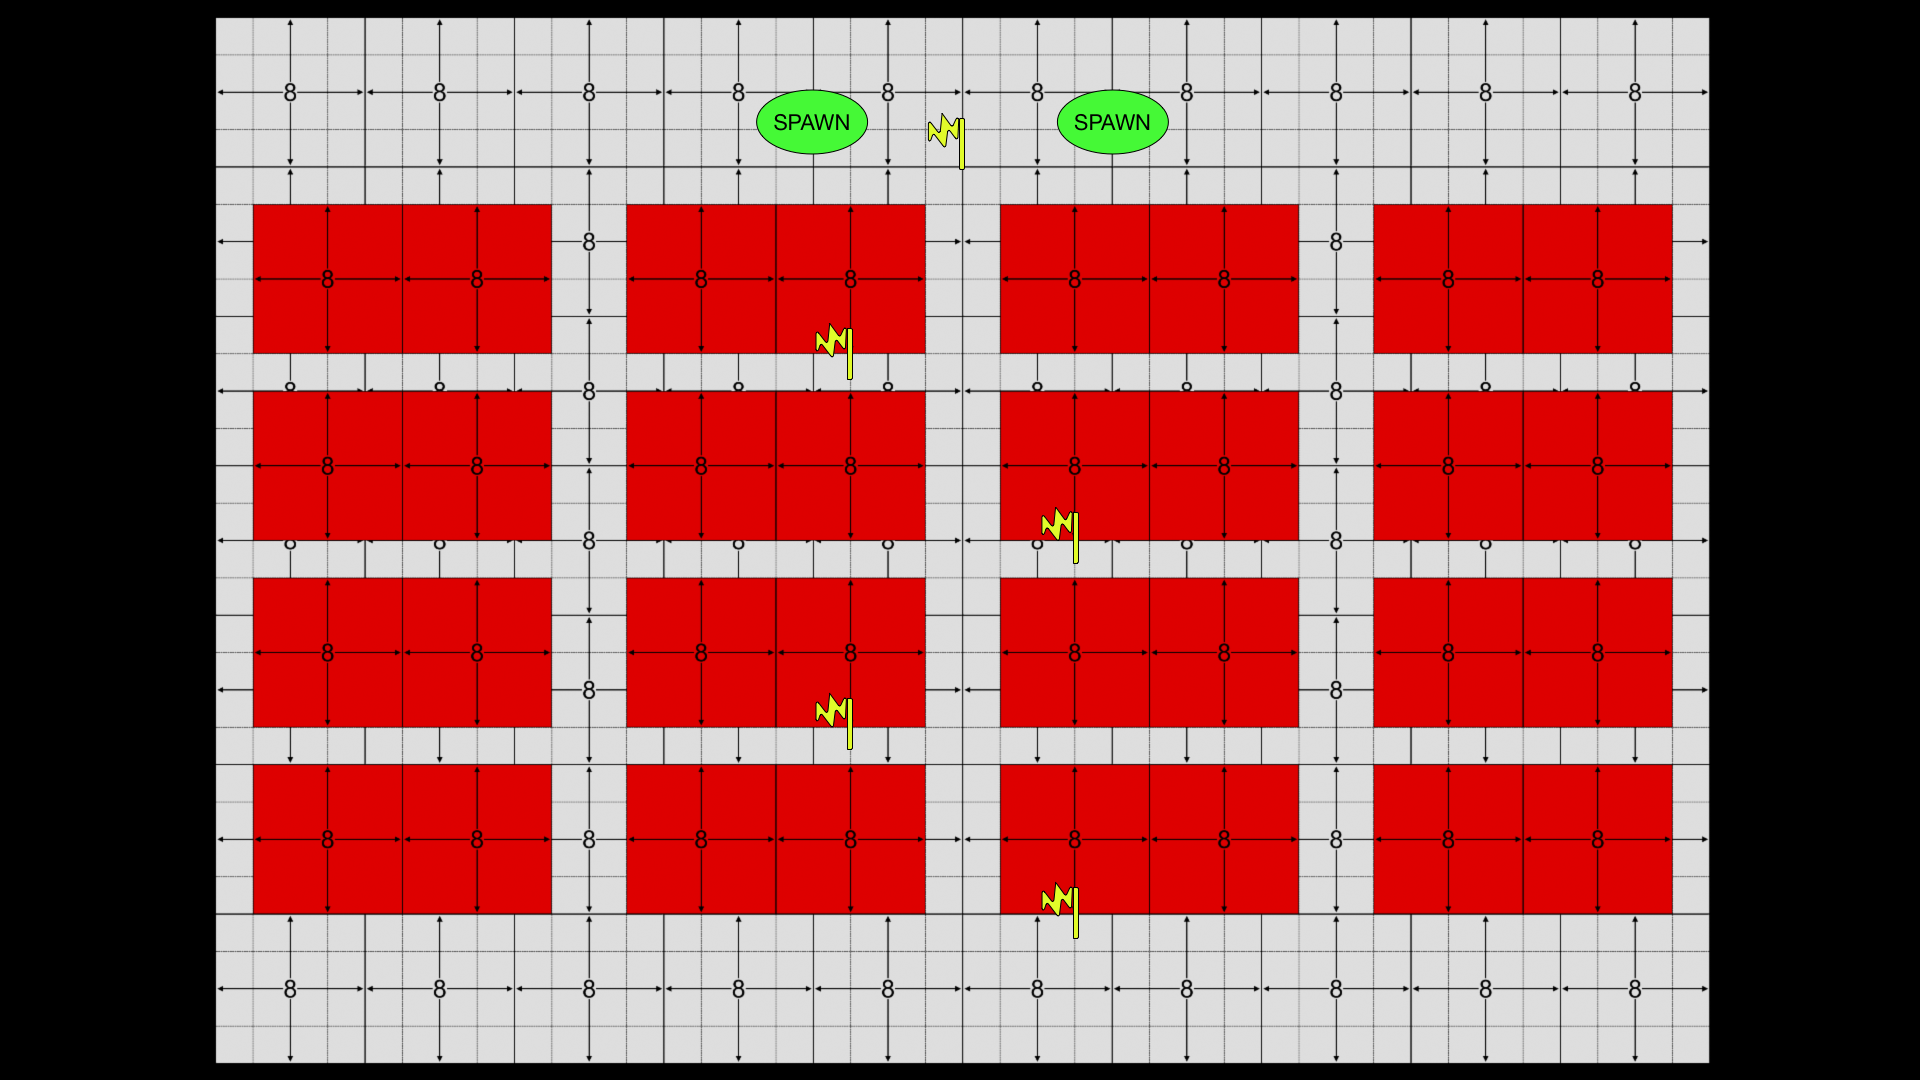
\includegraphics[scale=0.2]{taskoverview}
    \caption{Initial positioning of agents' starting points and resource markers.}
    \label{fig:x taskoverview}
\end{figure}
\section{Incorporating Genetic Programming}
The Genetic Programming module was built on top of FRAIL's existing features, substantially changing the ususal flow of execution to make it suitable for learning processes. Initialisation, evaluation and reproduction steps are all done internally, with evaluation being a step when the actual simulations are run. Since the population was being tested sequentially and the maximum time one could run was 20s (with the possibility to end early, in case all markers were gathered before that time), some testing would take more then 48 hours to complete. A decision was made to increase update frequency of the simulations tenfold, thus guaranteeing simulations would complete after maximum of 2s.
\subsection{Representation}
In the interest of avoiding integrity requirements and semantic incoherences (which would be undoubtedly caused by genetic operators), specimen are instances of a specialized class, separated from the actual Behavior Tree implementation. These trees are then parsed during evaluation step to an actual Behavior Tree that is injected to an AI Controller in the simulation.

This simplified implementation allowed for easier manipulation of the trees' components. The nodes are distinguished by their type, but otherwise have all parameters required to operate. While this poses a serious data redundancy, the possibility of freely adding additional node types and ease of operations made this option highly desirable.
\subsection{Genetic Operations}
\subsubsection{Initialisation}
The population starts as a set of randomly generated specimen of varying size and depth. Each tree generation starts with a random Composite node in root, then the decision is made a at each further step to either add a random Action / Condition node to current root's children or recursively create a random subtree, all bound by a maximum size and maximum depth allowed. This approach provides a varied population while maintaining good balance of Action / Condition and Composite nodes.
\subsubsection{Selection}
The selection method of choice is a regular implementation of Tournament Selection. At each step, a random sample of a given size is selected from the current population and sorted according to a fitness value of the specimen. The first individual from this set is selected for Reproduction purposes.
\subsubsection{Crossover}
On each iteration, two selected specimen have a chance (determined by crossover rate parameter) to produce two children which will be put into the next generation instead of them. The crossover itself is a single-point version, implemented as a exchange of randomly selected nodes (one from each tree) without minding their type nor location.
\subsubsection{Mutation}
Both available mutation methods were implemented: initially, only the possibility for the tree to undergo micromutation is tested - that is implemented by resetting randomly chosen node's parameters to a random values. However, each tree selected for a micromutation process (probability of which is dictated by a mutation rate) has a chance to undergo a macromutation process instead - that, in turn, is determined by a separate, macromutation rate. In this case, micromutation step is replaced entirely with ``Headless Chicken'' mutation.
\subsubsection{Fitness function}
Due to the format of the experiments, where solutions to two different scenarios were explored separately, used fitness function varied between experiments. There is, hovever, a number of factors that were considered relevant to the fitness of the specimen that can be presented now. These were:
\begin{itemize}
    \item \textbf{Number of markers gathered} - a number of resource markers gathered.
    \item \textbf{Time to completion} - how much time did it take to finish the simulation (i.e. how much time has elapsed untill all the markers were claimed).
    \item \textbf{Size of a Tree} - how many nodes were in the tree.
\end{itemize}
The first characteristic ended up being relevant only in the competitive scenario, where agents were to compete in claiming the markers: the number of claimed resources was, in fact, the defining characteristic. The relevance of the two following features, however, was common to both cases: the best solution is expected to finish the task as close to the shortest time as possible, while pressuring the algorithm to keep decreasing the size of a tree was done in the interest of both readability (and, with that, ease of modification) and execution time.
\section{Behavior Tree}
The solution produced by the algorithm had to be \textit{translated} to an actual Behavior Tree representation used in the simulations for the reasons discussed earler in this chapter. The process was, however, a part of the usual workflow and required no interaction from the user.

Specimen were built from only three kinds of nodes: \textit{Selector}, \textit{Sequence} and one Action - \textit{goToFlag(flagNumber)}. This decision was made based on relative simplicity of the task, not requiring elaborate choice in actions. \textit{goToFlag} autmatically chooses the optimal route to the selected path and, when the actor approaches capturing distance, attempts to claim the marker. Note that there is no information provided on the marker still being in the chosen place, as well as no knowledge at all about the state of the board. Agents operate thus in an environment with incomplete information, with the position of the markers being the only information available.

Furthermore, \textit{goToFlag} Action provided additional two variants, tied with the identifier argument. While values of 1-7 would select one of the existing markers, values $-1$ and $0$ held special meaning: -1 would set the course on the furthest \textit{available} (non-claimed) marker, while the latter would select nearest one. This was done in order to see if that level of abstraction would be preferable in certain situations, acting with critical timing against unchanging reference agent. The listing below presents pseudocode algorithm of \textit{goToFlag} Action.

\begin{lstlisting}
actionGoToFlag(int identfier) % e [-1, 7]
    if (identfier &==&  -1)
        goToFurthestFlag()
    else if (identfier &==& 0)
        goToNearestFlag()
    else
        goToFlag(identfier)
\end{lstlisting}
\section{Environment}
\subsection{Introduction}
\textbf{FRAIL} (Framework for AI Laboratories) is a platform developed in-house at Wroclaw's University of Technology (PWR) for purposes of testing artificial adversaries in shooter games. \cite{frailweb}

As an in-house project, users were able to freely access and change the source code, modifying existing controllers or creating new ones. Since its launch, FRAIL has seen use as a didactic aid during Artificial Intelligence classes and bootstrap for various AI-related projects, including evaluation by a video game development and publishing company, Techland for internal use. % citation needed?

In order to fully utilize the platform's capabilities, substantial changes have been made to FRAIL's engine in one of the previous projects, allowing for the entire process of Genetic Programming to be executed on the platform itself. A Behavior Tree implementation and representation related modules were taken from current version of FRAIL and the project was reverted to one of the earlier versions to reduce bloating. Genetic Programming module was implemented as a ``building block'' that could be placed on any map operating in ``Capture the Flag'' mode. Exploiting FRAIL's scripting behaviors and usage of RTTI (Run-Time Type Identification), a number of convenience changes were introduced to control the environment and algorithm parameters.
\subsection{Map overview}
The task planned for the agents can be described as a resource retrieval. To simulate this scenario, a map resembling a warehouse has been planned and prepared for use. Figure \ref{fig:x simmaprender} presents a 3D render of a finished map, while a top-down view, featured on Figure \ref{fig:x simmaptopdown} will be referred to further describe the design.

\begin{figure}[h]
    \centering
    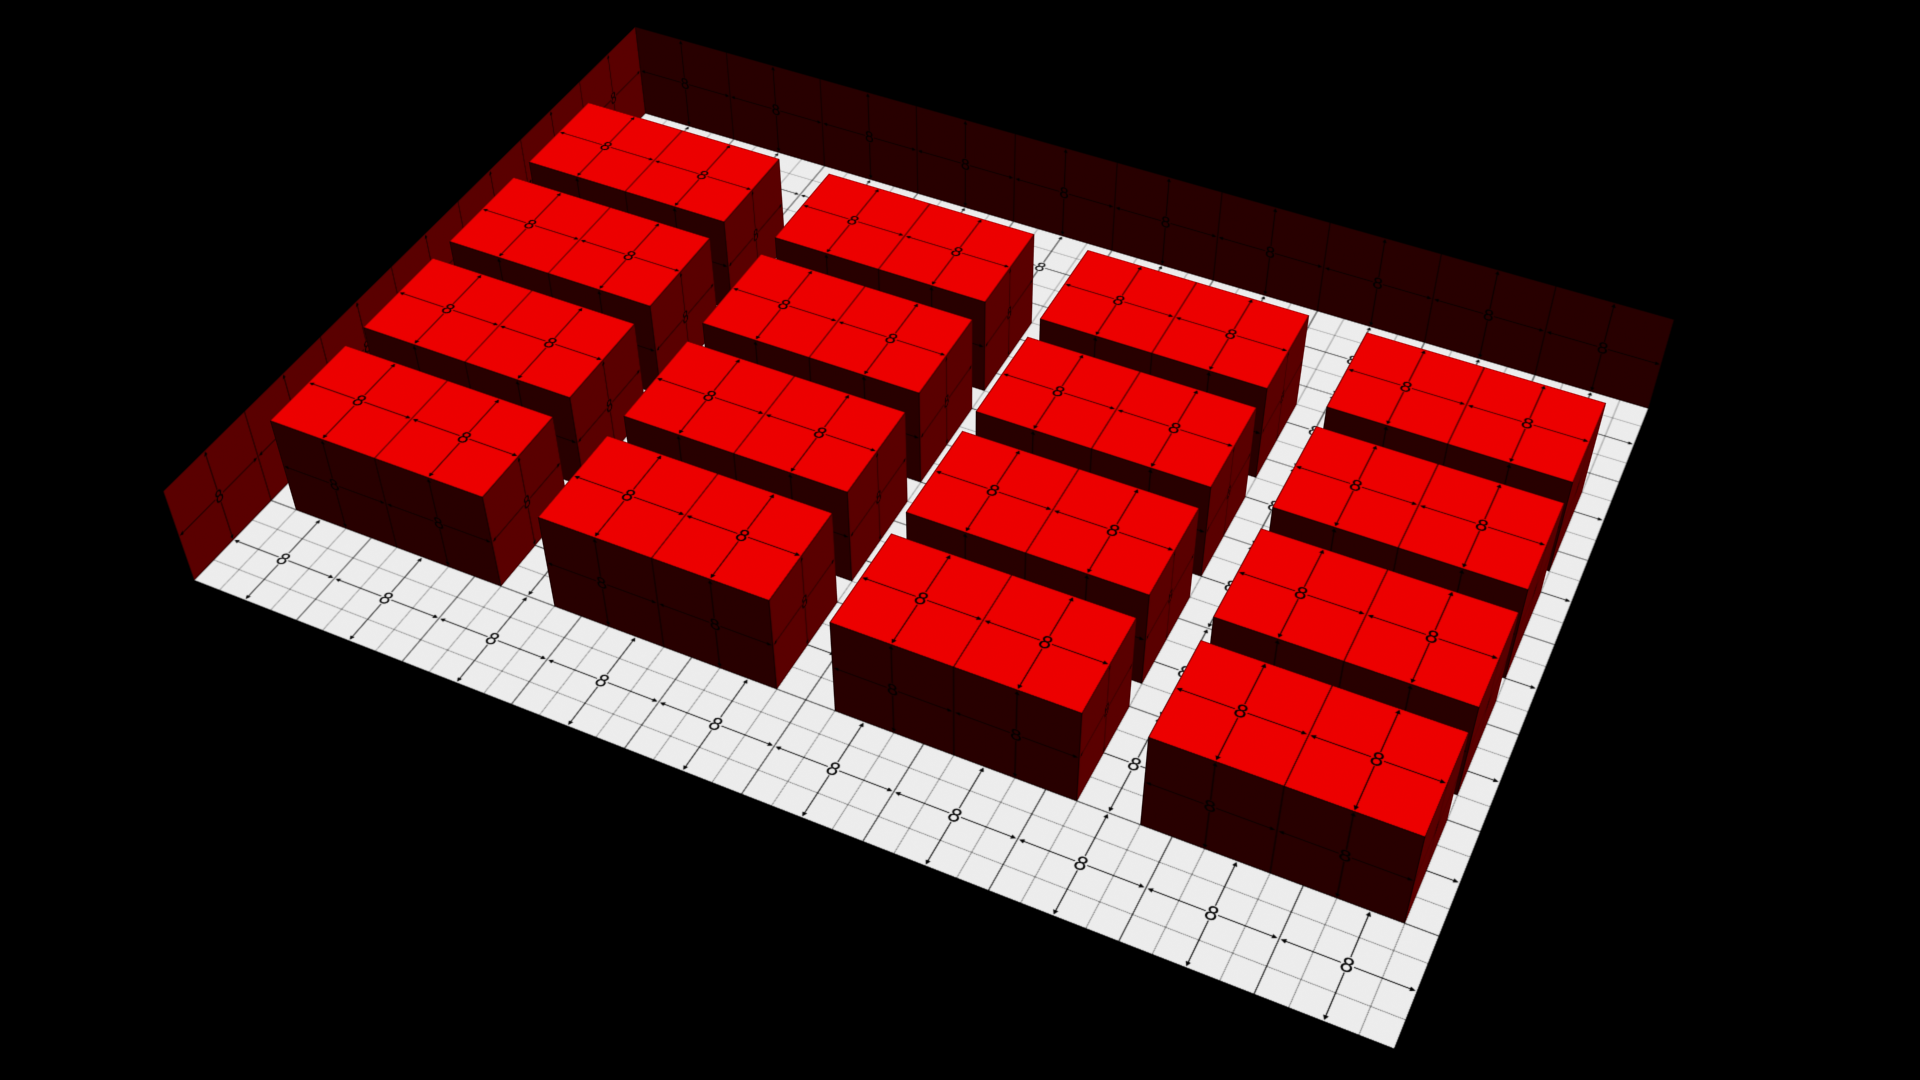
\includegraphics[scale=0.2]{frailmaprender}
    \caption{A rendering of scenery}
    \label{fig:x simmaprender}
\end{figure}

\begin{figure}[h]
    \centering
    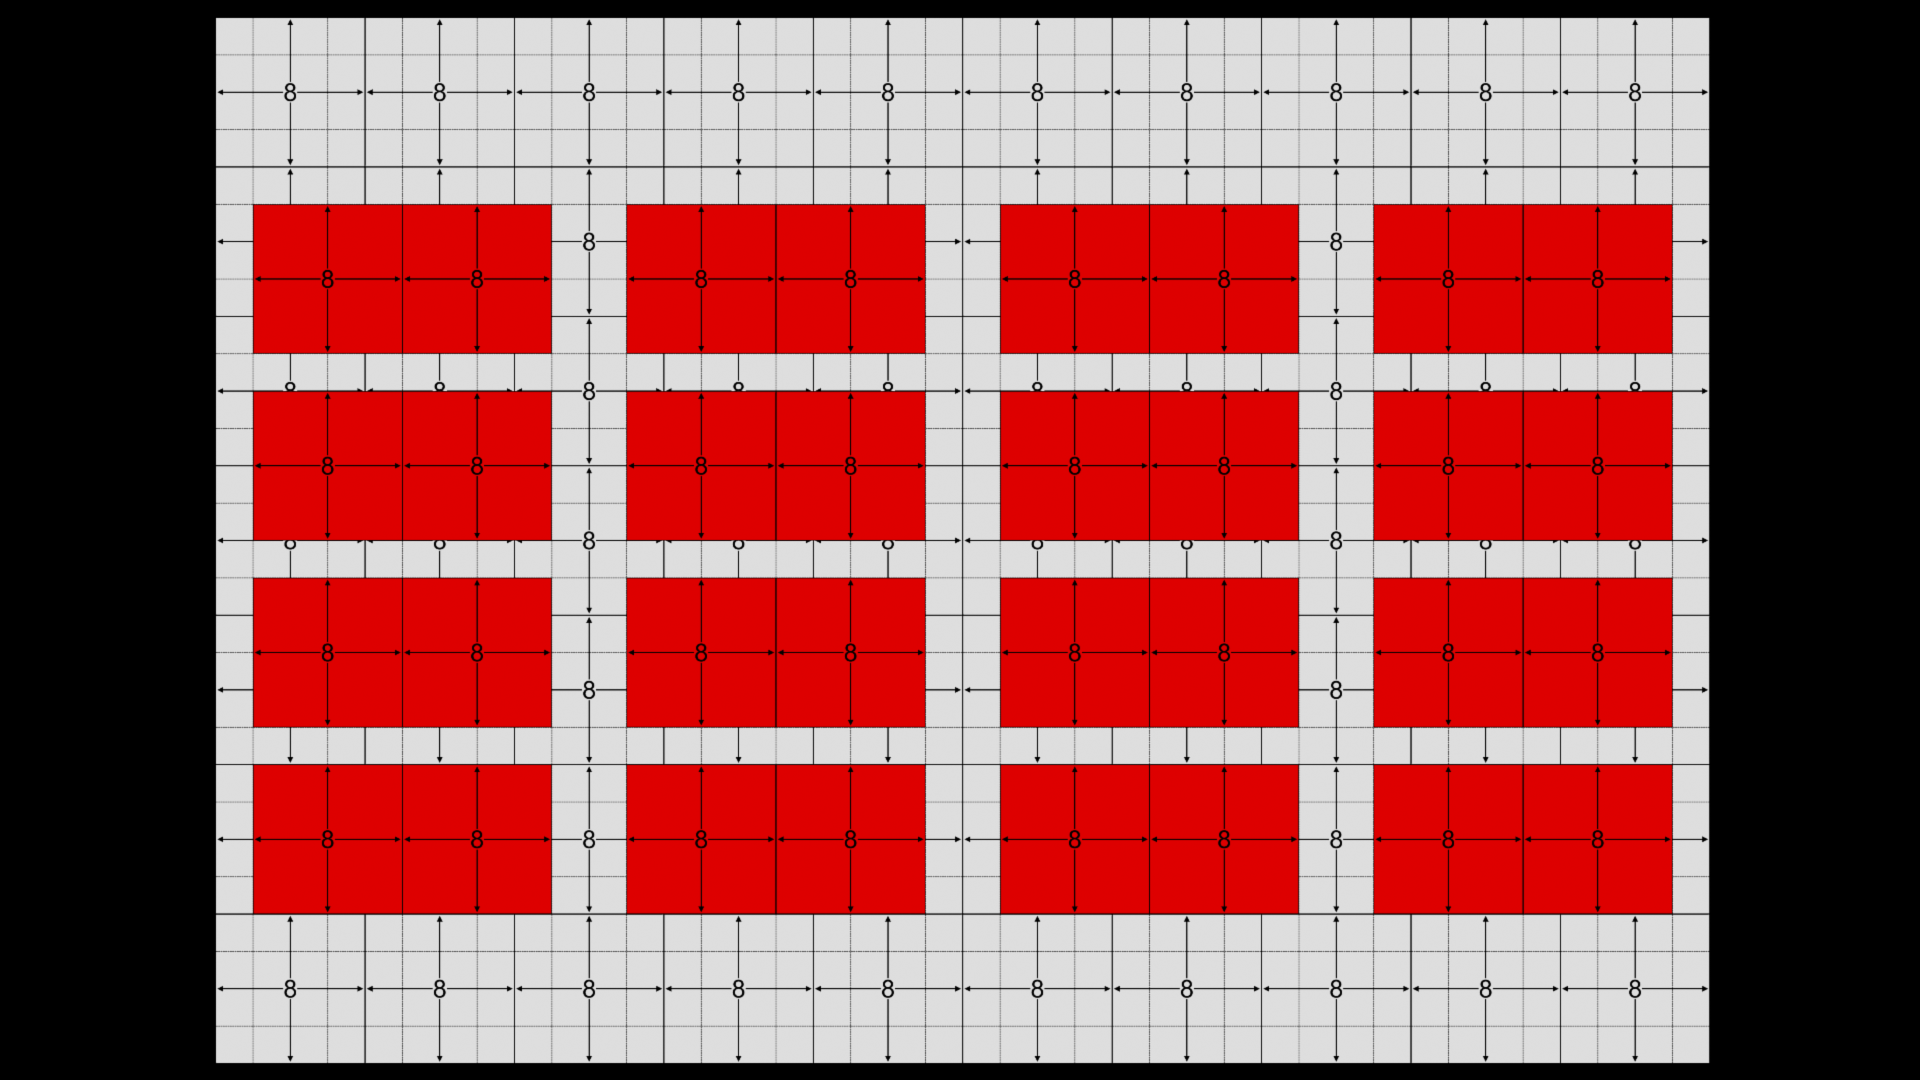
\includegraphics[scale=0.2]{frailmaptopdown}
    \caption{A top-down view of the map}
    \label{fig:x simmaptopdown}
\end{figure}

The map was designed with two to four agents in mind, with the possibility of scaling up when needed. Its shape is rectangular, measuring 80 on 56 simulation units. Over the middle section, 14 cuboid structures were placed symmetrically to act as storage containers / shelve-holding space, with access points along every edge. This placement allowed to make use of narrow alleys between containers in order to create potential conflict points, and positioning resources right next to them would hopefully allow for more faithful representation of a real-world resource gathering problem.
% I'm not sure what exactly belongs here. For instance: I should note that introduction of GP to the platform was done beforehand, since I made only the GP part, it was my partner who integrated it within frail. There were no publications, however, since it was only a class project.

\chapter{Results}
\label{chapter_results}
To learn how cooperative behaviors may influence success ratio in a particular task, the decision was made to first observe the evolution in case where agents work against one another, competing for a higher score. Only then, comparing the results with those of a cooperative case, conclusions regarding cooperation influence may be drawn.

The scenarios were tested in parallel with each change, were it to complicate the problem or put emphasis on certain components of the solutions.

The two scenarios shall be described in their dedicated sections below, focusing on key contrast points. Following, however, are the elements common to both cases.

Evaluation process of candidate solutions was made in the same environment, with identical starting points and resource markers' locations. In both scenarios, trees produced by Genetic Programming are accompanied by a unchanging, user-defined tree in the simulations. This reference agent uses one type of Action, \textit{goToFlag(flagNumber)}, visiting each resource marker in turn, capturing them from first to last, never changing path between simulations. Figure \ref{fig:x referenceagentdiagram} presents the Behavior Tree schematic of the reference agent. Existence of such tree could fill the function of both a pressuring component (reflected in the fitness function in the appropriate cases) and essentialy a time-gate, as gathering all markers would end the simulation. Furthermore, algorithms in both cases had access to identical Behavior Tree Components to build the trees from, thus ensuring equal sophistication of solutions in each scenario.

\begin{figure}[h]
    \centering
    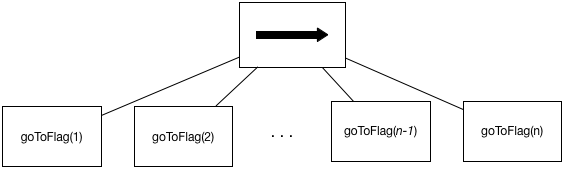
\includegraphics[scale=0.4]{referenceagentdiagram}
    \caption{A schematic of reference agent used in simulations.}
    \label{fig:x referenceagentdiagram}
\end{figure}
\section{Competitive Scenario Specification}
\subsection{Synopsis}
Competitive case assumed the optimal solution to the problem is maximizing the agent's personal gain. The markers gathered were counted for each agent separately, thus turning the task into a race - evolutionary agent was forced to get to as many markers as possible before the reference agent would claim them for himself.

After initial testing, the scenario was modified to feature 7 resource markers (instead of initial 5) and modified spawn points of agents -  readjusted to move evolutionary agent further back from the first marker. While increasing the number of markers served as an attempt to complicate the problem, moving evolutionary agent further from the first flag was done in the interest of being able to reproduce the results: since both agents were in the equal distance of the first flag and moved with the same speed, the matter of which one would claim the first flag was comparable to a coin-toss. Figure \ref{fig:x scenario1topdown} presents the final view of the competitive scenario map.

\begin{figure}[h]
    \centering
    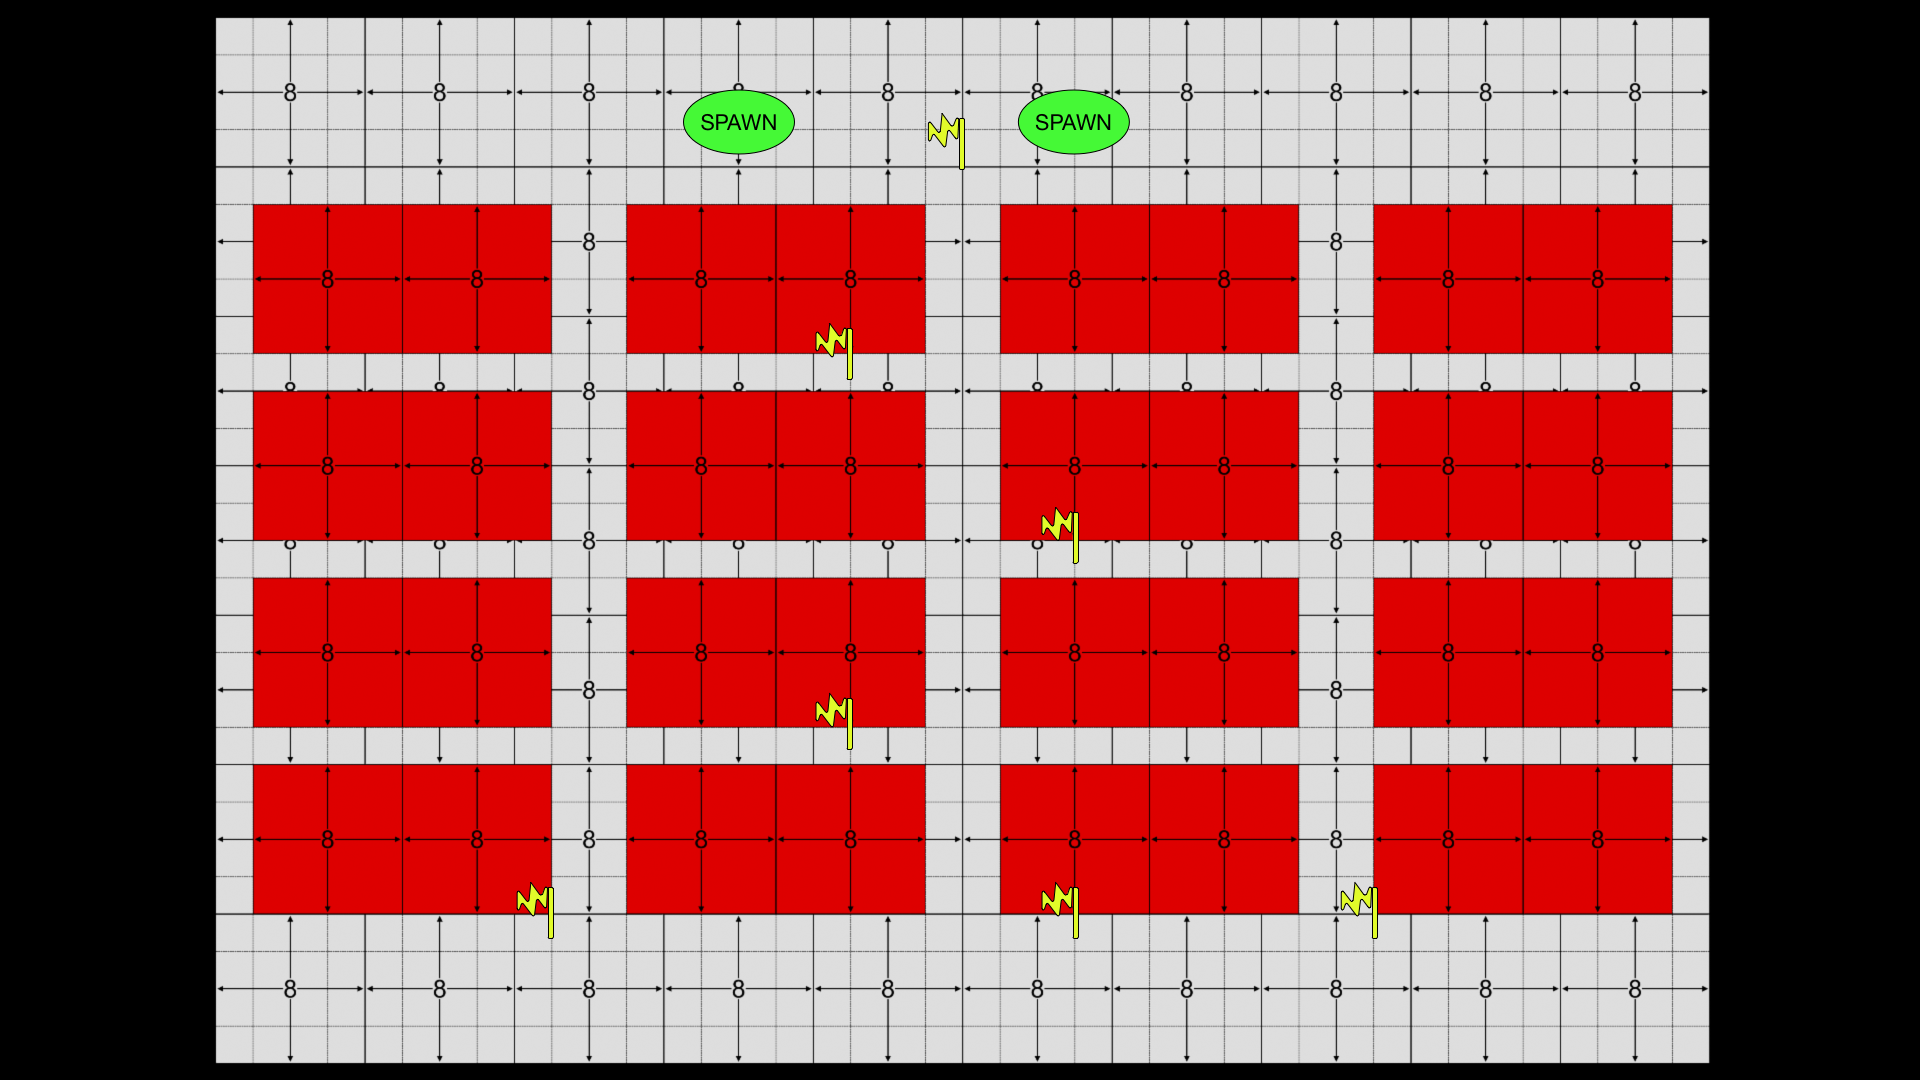
\includegraphics[scale=0.2]{scenario1topdown}
    \caption{Finished map of the competitive scenario environment}
    \label{fig:x scenario1topdown}
\end{figure}

\subsection{Fitness Function}
The competitive scenario is effectively a zero-sum game: a gain in utility of one agent means (prospective) loss of utility for the others. Considering that, the initial fitness value of the $i-th$ specimen in the population was a sum of $n$ markers gathered by an agent controlled by a tested tree, multiplied by a resource point constant $C_1$. This, however, wasn't feasible as a long-term solution. To introduce differentiability between the specimen scoring the same amounts of markers, a  factor of time in milliseconds multiplied by constant $C_2$ was then subtracted from the sum. Additionally, to coerce the algorithm into preferring smaller trees, a tree size factor with weight $C_3$ was further subtracted from this value. The finished formula for fitness function is presented on Equation \ref{eq:x scenario1fitness}.
\begin{equation}
    \label{eq:x scenario1fitness}
f(i) = C_1 * n - (\frac{t}{C_2} + \frac{s}{C_3})
\end{equation}
\subsection{Success Criterion}
\label{section_competitive_success}
With the goal of maximizing personal gain, which is the case with the considered scenario, desirable trees are those that claim every possible marker. However, since evolutionary agent's spawn position put it at the disadvantage (making it impossible to gather the first flag), only solutions with $n - 1$ flags gathered out of $n$ possible would be considered ``successful''. The true goal of a ideal solution was then to create a big enough difference in time taken to visit the markers, allowing it to reach and claim the last one.
\section{Cooperative Scenario Specification}
\subsection{Synopsis}
Cooperative scenario, in contrast to the ``selfishly'' motivated competitive one, takes a broader perspective. Instead of competing, agents were expected to work with each other towards claiming all 5 markers. However in time, the layout of the scenario was modified to maintain uniformity between the two cases' layout - that included both increasing the number of flags to 7 and modifying the agents' spawn positions - for comparison reasons.
\subsection{Fitness Function}
Due to competitive aspect being gone, a perspective on performance shifted substantially. The number of markers claimed by an agent became an impractical characteristic, with the time factor providing a much more considerable view on specimen performance. However, the decision was made to include the \textit{total number of markers} in the fitness function, serving as a constant, to ensure that the results from both scenarios are of the same order of magnitude. Aforementioned time and tree size components remained in untouched form, all the more critical in case at hand. Equation \ref{eq:x scenario2fitness} presents the fitness function used in evaluating specimen in cooperative scenario.
\begin{equation}
    \label{eq:x scenario2fitness}
f(i) = C_1 * (n + m) - (\frac{t}{C_2} + \frac{s}{C_3})
\end{equation} % legend?

\subsection{Success Criterion}
\label{section_cooperative_success}
In the cooperative case, the underlaying goal is to divide the markers between two agents in the most efficient way. To effectively operate, the desired outcome is achieving completion time shorter than the time it takes for the reference agent to complete his route. In other words, a successful solution will be able to successfully adapt itself to a potential partner's route and improve upon it in terms of time.

\section{Fitness Function Parameters}
The aforementioned point constants of the fitness function, defined as follows:
\begin{itemize}
    \item $C_1$ - resource marker point value
    \item $C_2$ - time factor weight
    \item $C_3$ - tree size weight
\end{itemize}
Were tuned by using \textit{grid-search} algorithm with a number of possible values of $C_2$ and $C_3$. $C_1$, however, remained unchanged. The decision was made that, for the purposes of the competitive case, the number of resource markers should remain the deciding factor.
The values of the parameters after grid-search tuning are presented in tables \ref{table:x tunedfitnessfunctionparameterscoop} and \ref{table:x tunedfitnessfunctionparameterscomp}.
\begin{table} [h]
    \centering
    \begin{tabular} {l r}
        \hline \hline
        Parameter Name & Parameter Value \\
        \hline
        $C_1$ - resource marker point value & 1000 \\
        $C_2$ - time factor weight & 0.1 \\
        $C_3$ - tree size weight & 100 \\
    \end{tabular}
    \caption{Selected Fitness Function factor weights for Cooperative Scenario}
    \label{table:x tunedfitnessfunctionparameterscoop}
\end{table}


\begin{table} [h]
    \centering
    \begin{tabular} {l r}
        \hline \hline
        Parameter Name & Parameter Value \\
        \hline
        $C_1$ - resource marker point value & 1000 \\
        $C_2$ - time factor weight & 0.01 \\
        $C_3$ - tree size weight & 10 \\
    \end{tabular}
    \caption{Selected Fitness Function factor weights for Competitive Scenario}
    \label{table:x tunedfitnessfunctionparameterscomp}
\end{table}
\section{Genetic Programming Parameters in Experiments}
After observing the results from a number of initial test runs as well as using \textit{grid-search} algorithm to help determine \textit{crossover rate}, \textit{mutation rate} and \textit{population size} parameters, the parameters used in the experiments are presented in table \ref{table:x selectedgpparameters}.

\begin{table} [h]
    \centering
    \begin{tabular} {l r}
        \hline \hline
        Parameter Name & Parameter Value \\
        \hline
        Maximum Number of Generations & 100 \\
        Population Size & 200 \\
        Crossover Rate & 25\% \\
        Micromutation Rate & 15\% \\
        Macromutation Rate & 2\% \\
        Tournament Selection Tourney Size & 10 \\
    \end{tabular}
    \caption{Selected Genetic Programming parameter values.}
    \label{table:x selectedgpparameters}
\end{table}

After a number initial runs, it was clear that keeping a maximum number of generations above one hundred served no function - there were no instances that did not converge before that point and following were long periods of stagnation or, even worse, loosing best specimen. The method responded positively to increasingly higher number of specimen in the generation: totaling at 200, this ensures a good variety of genetic material for the algorithm to make use of. Crossover and mutation rates were kept low due to the risk of destroying relatively low number of good specimen each generation. On the other hand, they could not have been set \textit{too low}, lest the algorithm would not explore the search space properly. It is worth pointing out that macromutation (``Headless Chicken'') was kept at extremely low occurrence chance specifically for that reason - there weren't any instances suffering from too early convergence, something that macromutation would have been a remedy to. Choosing a 5\% value of tourney size ensured it would still be possible to get specimen with mid-range fitness value into the next generation while keeping the selection pressure relatively high.

Table \ref{table:x selectedbtparameters} presents selected parameters used during tree generation steps in the algorithm.
\begin{table} [h]
    \centering
    \begin{tabular} {l r}
        \hline \hline
        Parameter Name & Parameter Value \\
        \hline
        Maximum Tree Depth & 6 \\
        Starting Generation Minimum Tree Size & 20 \\
        Starting Generation Maximum Tree Size & 30 \\
        Headless Chicken Generated Tree Minimum Size & 10 \\
        Headless Chicken Generated Tree Maximum Size & 20 \\
        Headless Chicken Maximum Tree Depth & 5 \\
        Expected \textit{Action-to-Composite} node Ratio & 3:1 \\
    \end{tabular}
    \caption{Selected Behavior Tree generation parameter values.}
    \label{table:x selectedbtparameters}
\end{table}
The tree related parameters were chosen after a careful consideration of desirable feats both in the initial generation as well as during rarely-observed macromutation. Generating the tree between 20 and 30 nodes would create a varied populations with different shaped trees, while maintaining decent complexity bound by maximum tree depth. The need for larger number of Actions in relation to Composite nodes was dictated by a simplicity of the task and in the interest of further coercing the algorithm to prefer simpler structures.
\newpage
\section{Exemplary Specimen}
In this section, a sample specimen representation is presented and described. The listing below presents the text representation of a tree, while figure \ref{fig:x exemplaryspecimenscenario1} contains a (arguably) more human-readable form.
\begin{lstlisting}
Sequence
  ActionGoToFlag 0
  ActionGoToFlag 3
  ActionGoToFlag 4
  ActionGoToFlag 4
  Selector
    Sequence
      Selector
        Sequence
          ActionGoToFlag 7
          ActionGoToFlag 5
          ActionGoToFlag 6
        ActionGoToFlag 6
      ActionGoToFlag 0
      ActionGoToFlag 3
      ActionGoToFlag 4
    ActionGoToFlag 3
    ActionGoToFlag 7
  Sequence
    ActionGoToFlag 2
    ActionGoToFlag 3
  ActionGoToFlag 4
  Selector
    ActionGoToFlag 1
    ActionGoToFlag 1
  ActionGoToFlag 5
  ActionGoToFlag 2
  ActionGoToFlag 3
\end{lstlisting}

\begin{figure}[h]
    \centering
    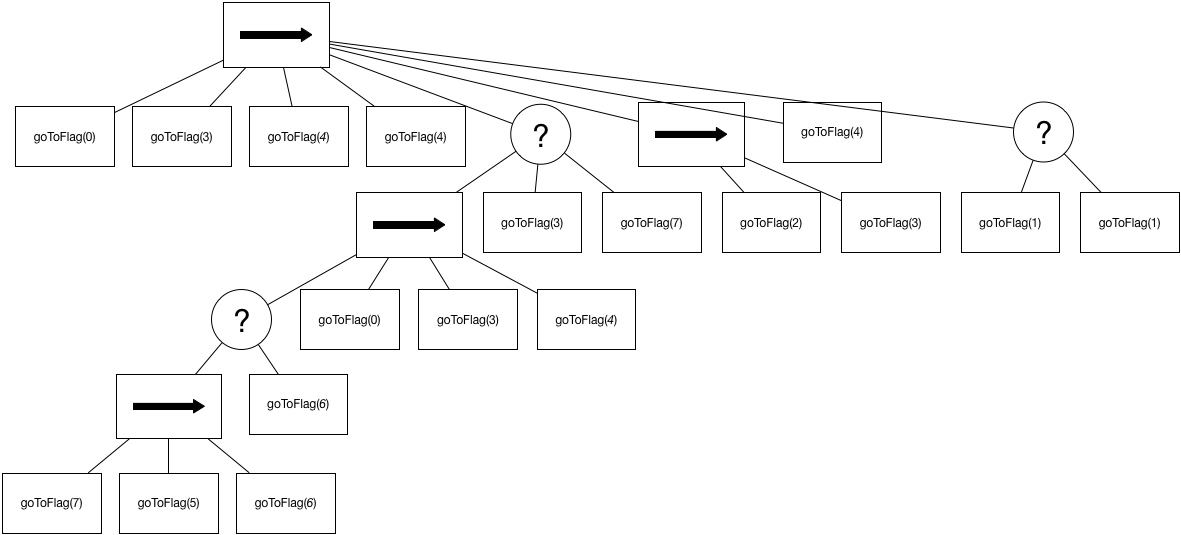
\includegraphics[scale=0.4]{exemplaryspecimenscenario1}
    \caption{Example diagram of a evolutionary generated specimen.}
    \label{fig:x exemplaryspecimenscenario1}
\end{figure}

This particular specimen was generated during one of competitive scenario experiments and his evaluation placed it on value 5911. Knowing both the value of fitness value constants it can be proven that the specimen claimed 6 resource markers out of 7 possible.

The tree has a very cluttered look and many unnecessary placed nodes, but the route should be clear: going from the top, it's going to visit the closest marker, which is the second one (sic!), then the third, proceeding to the fourth one (twice, in fact, but the second call will return instantly) and head for the last one, only to return to the fifth and sixth, probably meeting a reference agent nearby fifth marker. The rest of the nodes, as mentioned before, serve no function in this particular scenario. Unfortunately, the tree didn't follow the expected strategy (gaining a bit on each marker only to make a final push from sixth to seventh) instead opting to devise a new one. Although - as seen above - the strategy of choice seems to be at least equally viable.
\section{Optimization Results}
In this section, results of model cases (one from each scenario) will be presented. When analyzing the results, following factors were considered:
\begin{itemize}
    \item The shape of the algorithms' best specimen fitness value curve and its relation to average fitness value one.
    \item An average size of a tree throughout the iterations.
    \item Difference in node count from a \textit{minimal} successful solution % reword? Clear enough?
    \item A number of iterations needed for the best specimen to achieve success.
\end{itemize}
The shape of fitness plots indicate the general state and health of the Genetic Programming algorithm. While the plot indicating top fitness value in the population is certainly important (the success measure is directly tied to a top specimen), it's the average fitness value in the population that provides the much needed information on population growth, stagnation or even oscillations, indicating local plateaus.

The average size of a tree is also a useful indicator of a general perceived value of the generation: while larger trees are not necessarily always worse (since the execution time of a tree is virtually negligible), they most definitely contain needless constructs. Apart from being nigh unreadable, disregarding tree size would certainly result in need of introducing post-processing to prune a number of never-to-be-executed branches.

The task was designed in a way allowing for the optimal solutions to be relatively simple in structure: such solution, written manually, would be composed of no more than 7 (in competitive scenario) or 5 nodes (in cooperative one). These solutions would be deemed \textit{minimal}. Since tree size is one of the factors determining a specimen fitness, it is reasonable to expect the algorithm to converge on a tree that is close to that size.

Finally, the number of iterations needed to produce a first solution that is deemed ``successful''. Looking into the matter from the user's perspective,the only feasible characteristic is the speed of achieving a \textit{fit} specimen, able to deal with the task at hand with given restraints.

Figure \ref{fig:x competitivefitnessplot} presents a plot of the highest fitness value and average fitness in the population in respect to iteration in the competitive scenario. Figure \ref{fig:x competitivetreesizeplot}, however, illustrates the change of average tree size in the population in the course of the algorithm's run in the same scenario.

\begin{figure}[h]
    \centering
    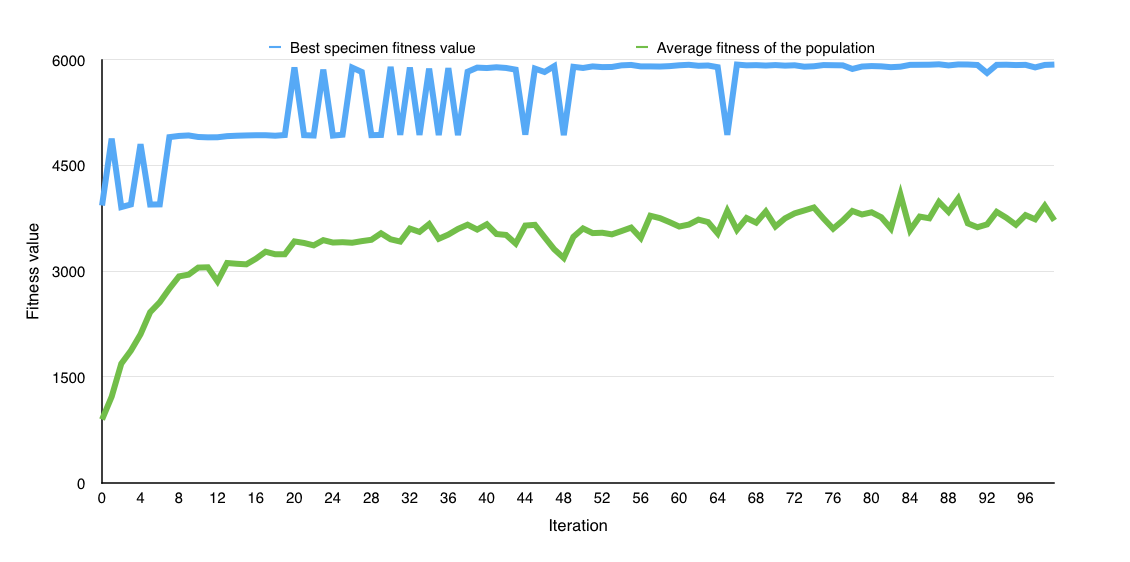
\includegraphics[scale=0.6]{competitivefitnessplot}
    \caption{A fitness value with respect to iteration plot in the competitive scenario.}
    \label{fig:x competitivefitnessplot}
\end{figure}

\begin{figure}[h]
    \centering
    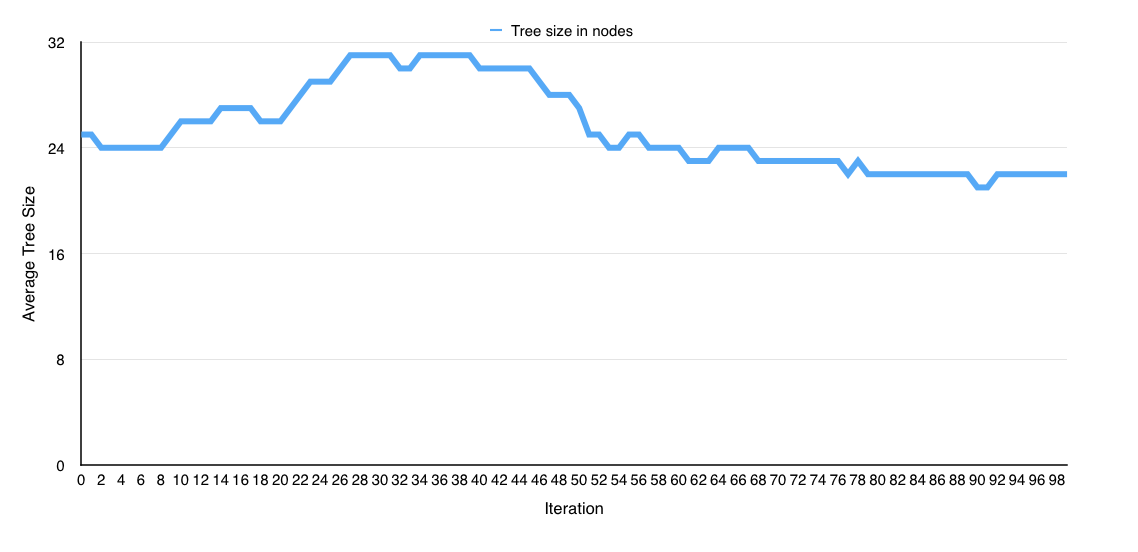
\includegraphics[scale=0.6]{competitivetreesizeplot}
    \caption{An average tree size with respect to iteration plot in the competitive scenario.}
    \label{fig:x competitivetreesizeplot}
\end{figure}
The algorithm's run in this particular case started on a relatively high note, with the best specimen claiming 4 markers for himself. In the next few iterations, best fitness achieved increased, then oscillated around 4200 value, to finally stabilize on a value closer to 5000. Up to this point, one can see the average fitness in the generation rising, indicating that, while there were no radical increases in value, the algorithm was producing more and more feasible candidates. Then, surely due to particularly good mutation or crossover operations, a breakthrough was made and the population achieved first successful specimen in the run. This one, however, was instantly lost, having not been copied over to the next generation. The curve then starts oscillating heavily, with the algorithm producing further successful specimen only to lose them few cycles later. Finally, around iteration 50 mark, the best specimen was kept for a longer duration. Note that the first successful individual marked the decline in average fitness growth, meaning that by that time, the population has been saturated with useful gene structures.

The size plot is intended to be considered and analyzed together with the fitness values. Having done that, one can observe that with the first successful specimen produced, the population started intensively increasing in node count. Having achieved large enough pool of fit solutions, size started to be the differentiating factor, successfully lowering the number. This is the perfect example of larger trees being promoted in the initial stages (since bigger trees have a higher chance of containing a useful node structure combination), but having their value decreased as the useful genes from them are passed into further generations. This also poses an balance question - whether the first found successful specimen should be accepted, or will processing more generations rewarding?

\begin{figure}[h]
    \centering
    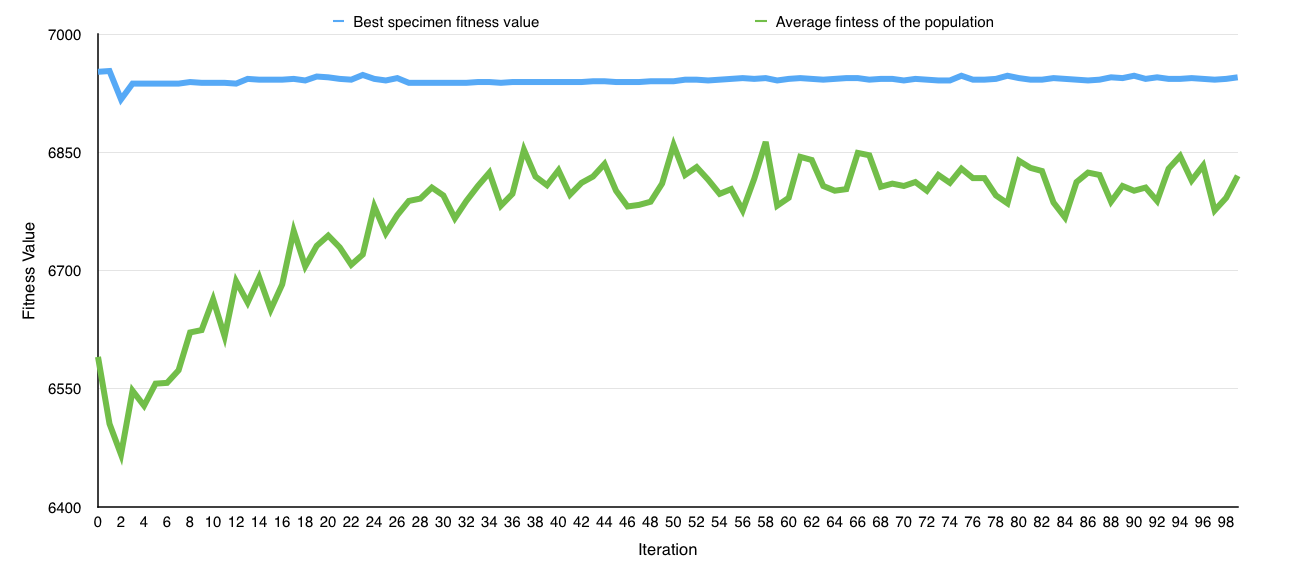
\includegraphics[scale=0.6]{cooperativefitnessplot}
    \caption{A fitness value with respect to iteration plot in the cooperative scenario.}
    \label{fig:x cooperativefitnessplot}
\end{figure}

\begin{figure}[h]
    \centering
    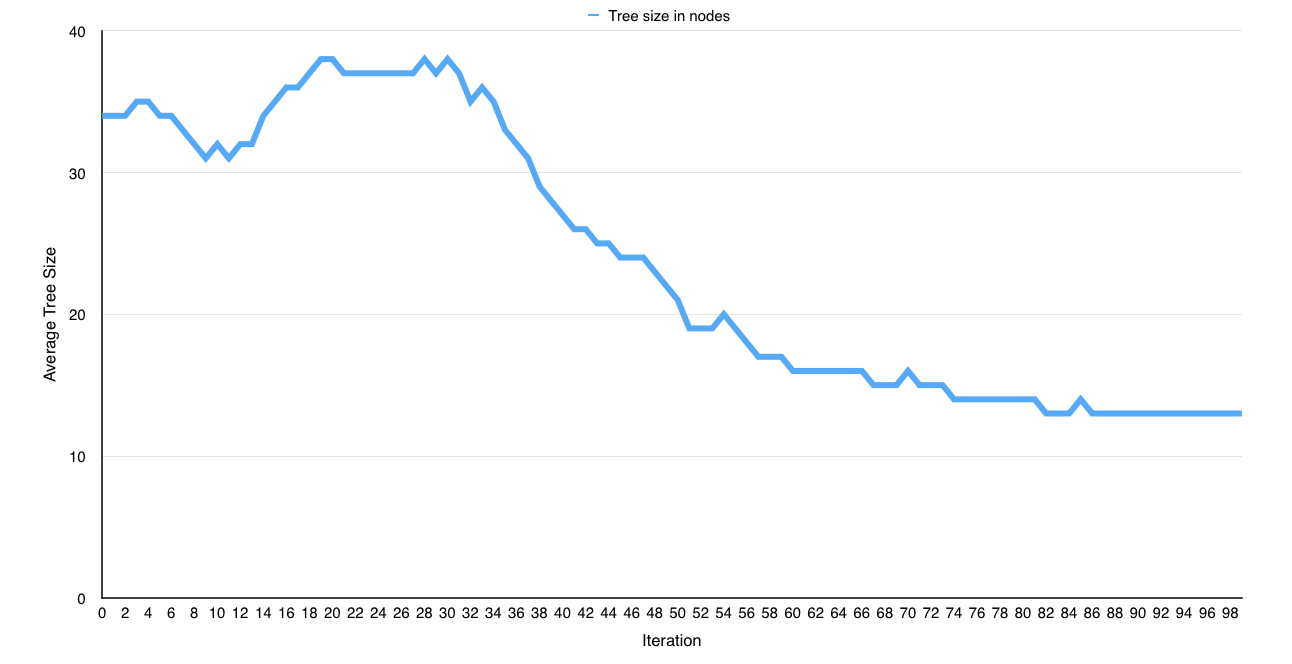
\includegraphics[scale=0.6]{cooperativetreesizeplot}
    \caption{An average tree size with respect to iteration plot in the cooperative scenario.}
    \label{fig:x cooperativetreesizeplot}
\end{figure}

Compared to the competitive scenario, the fitness plot in figure \ref{fig:x cooperativefitnessplot} presents much \textit{calmer} best fitness curve with no sudden changes in value, although with oscillations in abundance. Having produced a successful specimen in the first generation, the individual is instantly destroyed, its genes diluted in the pool of next generation. Another one, however, is produced as quickly as the fourth generation of the algorithm. The best specimen value starts oscillating with low amplitude, stabilizing after a good while. Average fitness value curve reflects that progress well, with the oscillations starting only when the other one stabilizes (again, marking the point where the population is saturated).

The progress of the population in the cooperative scenario is definitely more visible on figure \ref{fig:x cooperativetreesizeplot}. On 30th generation, when the fitness value of the best specimen appears to enter stagnation, abrupt decrease of an average specimen node count begins. Over the next 50 iterations of the algorithm, the average size is reduced almost thrice - from 36 nodes to 13.

While the average tree size of the population is an important indicator of the algorithm's overall health and progress (in a sense, since the progress can be presented as the ratio of current node count to the \textit{minimal solution} node count), it's the size of a best specimen tree that's important for the potential end-user. Figure \ref{fig:x competitivebestspecimentreesizeplot} presents the changing of the size of the best solution with regards to generation from one of the later experiments with increased tree size factor weight.

\begin{figure}[h]
    \centering
    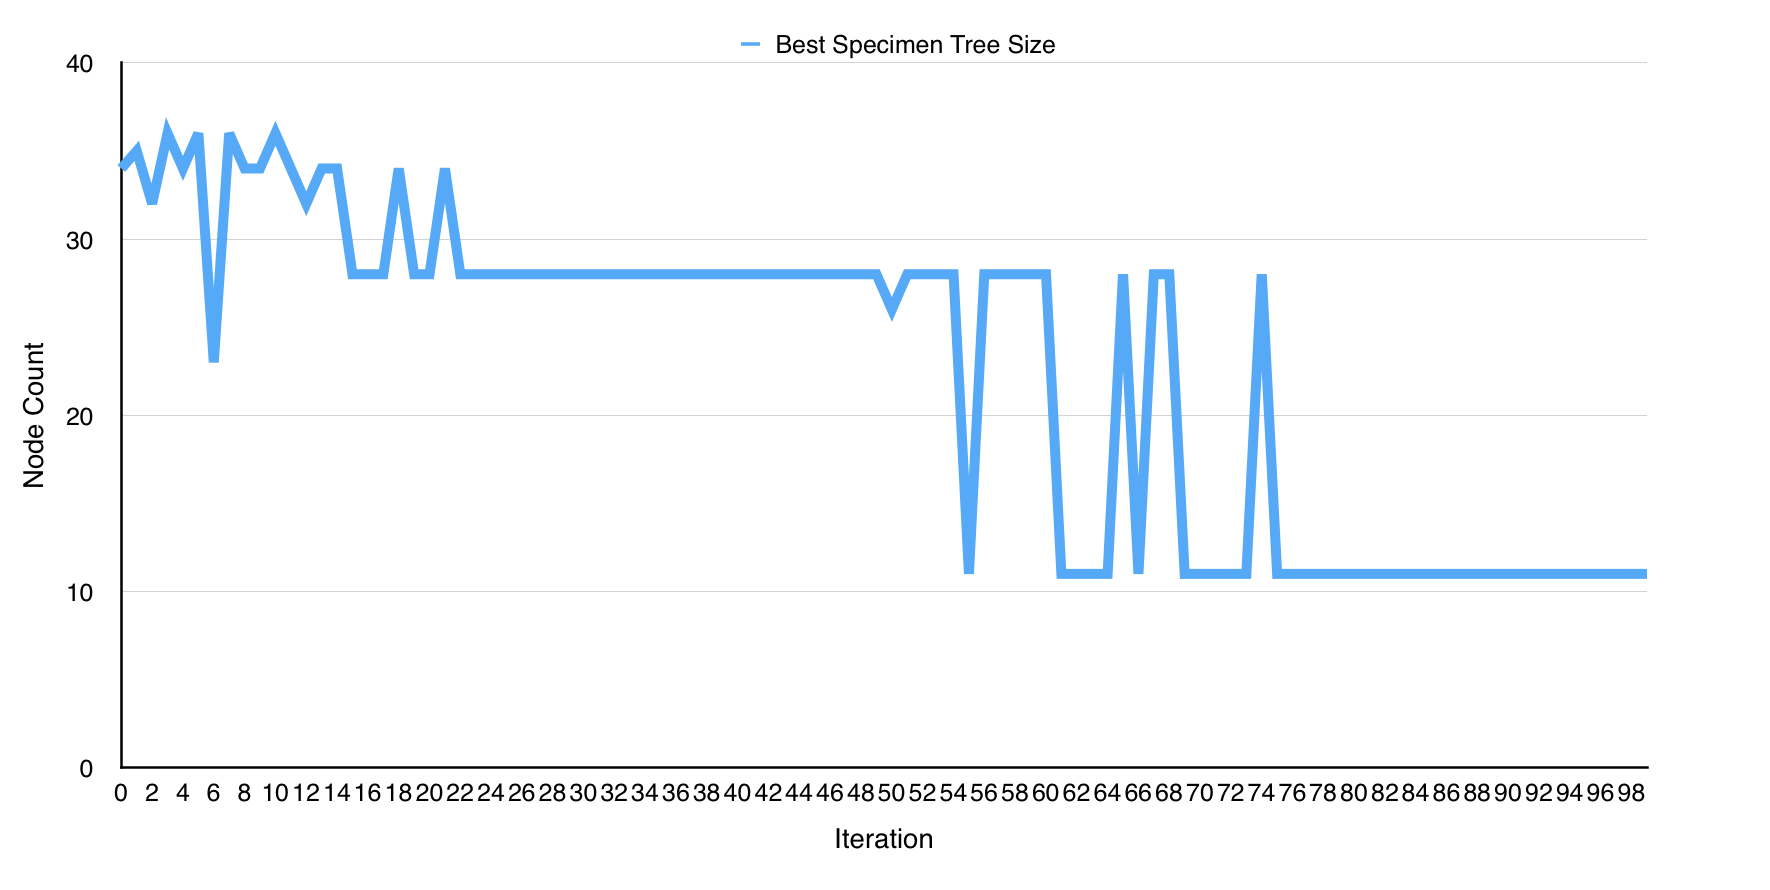
\includegraphics[scale=0.4]{bestspecimentreesizecomp}
    \caption{A best specimen tree size with respect to iteration plot in the competitive scenario.}
    \label{fig:x competitivebestspecimentreesizeplot}
\end{figure}

The relation between the size of the best specimen tree and the average tree size of the population can be compared to one between best specimen fitness value and average fitness of the population - the first few generations are a space for experiments, where size itself isn't more important than ever decreasing time. After coming up with a sufficiently big pool of good combinations of nodes, the decrease in size begins. 28 nodes is established as a size as early as 20th iteration, staying that way till generation 52, where the plateau is broken and, through a 20-generation oscillation cycle, new local optimum is reached.

Figure \ref{fig:x cooperativebestspecimentreesizeplot} presents identical changes, but experienced in cooperative scenario.
\begin{figure}[h]
    \centering
    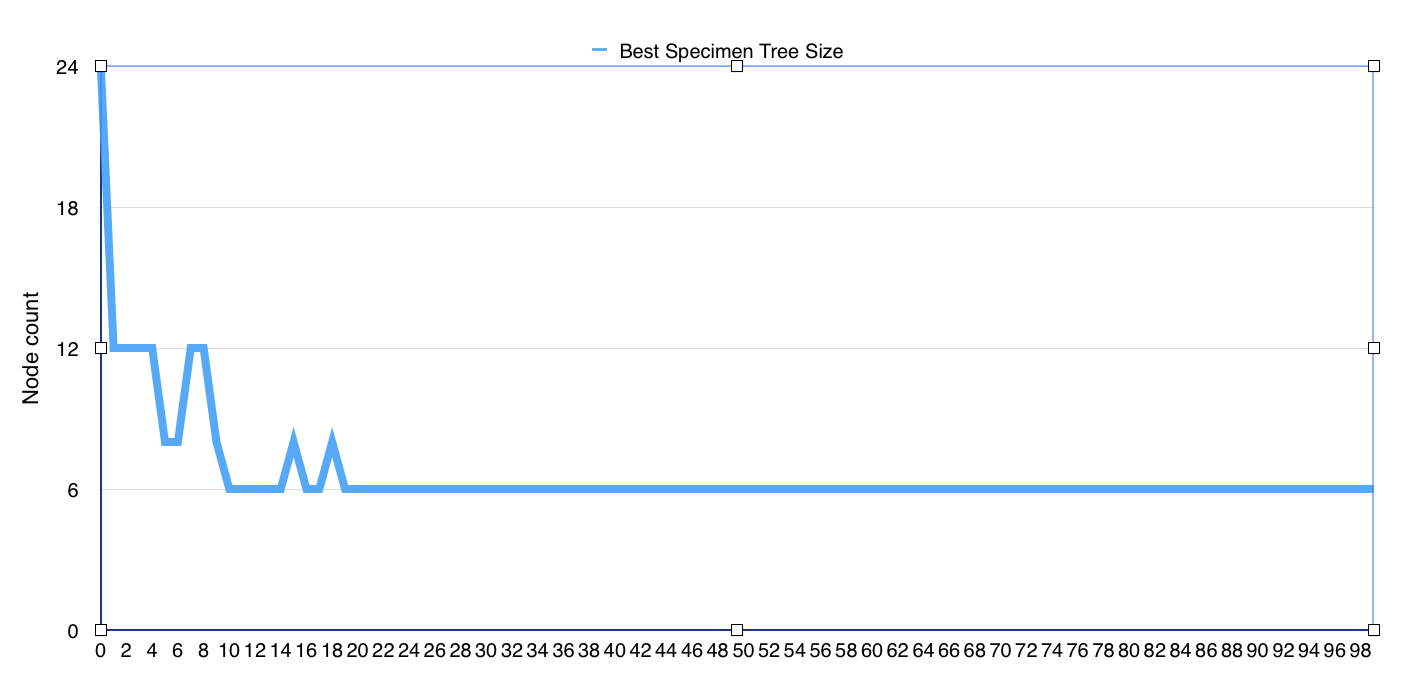
\includegraphics[scale=0.5]{bestspecimentreesizecoop}
    \caption{A best specimen tree size with respect to iteration plot in the cooperative scenario.}
    \label{fig:x cooperativebestspecimentreesizeplot}
\end{figure}
The decrease in node count in cooperative scenario is much more sudden - tree size had 10 times more influence on the fitness value of the specimen compared to competitive case (Table \ref{table:x tunedfitnessfunctionparameterscoop} for cooperative case, Table \ref{table:x tunedfitnessfunctionparameterscomp} for competitive case). With that large influence from the start, it is not unusual that the node count drops twice between the first and second generation. The decrease is sustained through the further generations (not without few slip-ups, when the best specimen was dropped from the population) to stabilize on 19th iteration.
\section{ Larger Scale Results } % this needs to change. Extended experiments?
To gain insight on how the algorithm approaches the two scenarios, we decided to compare the results of multiple executions. Given that the one full run of the algorithm takes 20 000 simulation runs, we decided to distribute the testing over 10 computers, each capable of running two instances of our application at once without loss of performance. The pace of the simulations was also adjusted to 3 times the regular speed to increase the number of results achieved in a reasonable time.

Overall, we were able to gather 50 results per case (cooperative \& competitive).

\chapter{Conclusions and Future Work}
\label{chapter_conclusions}
In this thesis, we aimed to answer the question:  ``How selfish and utilitarian behaviors between artificial agents influence the learning efficiency in task-oriented environments?''.

In order to simulate the agents' motivations, we designed a task that could be solved while puting agents against each other or allowing them to work together, while being simple enough for the results to be readable and for the optimal solution easily imaginable. We then designed a way to grade them, simulating a cooperative or competitive environment working against (or teamed with) a static opponent. Finally, we performed experiments on a bigger scale to see how the two approaches compare. To perform the comparison itself, we defined succes criteria based on our emirical data gathered so far. The algorithms in a competitive scenario produced a successful specimen after 100 generations in 50\% of the cases. The algorithms teaching competitive agents, however, achieved 78\% success rate after the same number of generations. Examining the size component, we noted 70\% success rate across the results from the cooperative case, with 22\% of the algorithm runs fulfilling that criteron in competitive scenario.

Based on the results, we can conclude that the speed at which the two approaches progress differs between stages of learning - changing it pace after certain local optima. Given the fact that the near-optimal solution observed is smaller than in cooperative scenario, we expected it to evolve sooner and in a greater numbers - that, however, did not happen.

We consider comparing the two approaches the main contribution of this work. Additionally, while achieving the thesis goal, we created a reliable platform for experiments using Genetic Programming and Behavior Trees, both separately and together. The effects of problematic areas in joining Behavior Tress with Genetic programming were partly contained by adding additional clauses to tree generation and crossover.

Future work will attempt to verify and expand on the results achieved in this thesis, especially in matters of increasing the scale of reseach and defining proper error measurements to confirm or disprove our current results. That said, the work here merely touches the surface of genetically evolving Behavior Trees and the behavior types they might exhibit. A direction we intend to focus on is a deeper analysis of the population - with greater insight on what structure do the specimen tend to create in various stages of the algorithm, it might be possible to incorporate the group selection ideas based on kinship or similarity of the specimen, mentioned in \cite{cooperationevolution}. Furthermore, developing more sophisticated methods of crossover and mutation, aware of constraints of Behavior Tree encoding, would naturally increase the effectiveness of evolving such trees. The concept of adaptation of the agent to a given environment should also be explored. The task considered in this thesis - arguably simple - has ben proven to be solvable with the simpliest of elements. A natural next step would be increasing both the dificultness of the problem and the resources available to the algorithm.


\printbibliography
\end{document}
